% Pour toute question sur l'utilisation de cette classe, écrivez à jerome.soucy(at)ulaval.ca
% Nécessite la classe Evaluation.sty dans le même dossier ou dans le PATH de votre système
% Nécessite le fichier logo_ul.pdf dans le même dossier un dans le PATH de votre système
\def\Ponderation{40}
\def\SigleNumero{STT-1900}
\def\NomCours{Méthodes statistiques pour ingénieurs}
\def\DateEvaluation{21 octobre 2022 de 18h30 à 21h20}
\def\Session{Été 2021}
\def\NomEvaluation{Examen 1}

% Ne rien mettre entre les accolades si l'enseignant (ou l'enseignante) est aussi le coordonnateur (ou la coordonnatrice)
\def\Coordonnatrice{}
\def\Coordonnateur{}

% Ne rien mettre entre les accolades s'il y a plus d'une section
\def\Enseignant{}
\def\Enseignante{}

% Ne rien mettre entre les accolades s'il s'agit d'un cours à section unique
% Mettre le nom de chacun des enseignants et enseignantes entre les accolades
% Une case à cocher sera générée pour chacune des sections
\def\SectionA{Audrey-Anne Vallée}
\def\SectionB{Abderazzak Mouiha}
\def\SectionC{}
\def\SectionD{}

% Concerne seulement les travaux pratiques : écrire entre les accolades le nombre maximal de membres pour une équipe
\def\NombreLignes{}		

% Si vous souhaitez qu'apparaisse une déclaration d'honneur au bas de la première page, écrivez quelque chose entre les accolades
\def\EnLigne{}

\def\Directives{
	\begin{enumerate}
			\item Matériel autorisé:
		\begin{itemize}
		    \item Calculatrice scientifique {\bf autorisée par la faculté des sciences et de génie};
		    \item Une seule feuille aide-m\'emoire \textbf{manuscrite} de format lettre (8.5''$\times$11'') recto-verso.
		    \end{itemize}
		\item Assurez-vous que cette \'evaluation comporte \numquestions ~questions réparties sur \numpages~pages, pour un total de \numpoints \ points.\
		\item \textbf{Veuillez ne pas débrocher votre examen.}
		\item Les tables de lois se trouvent à la fin du cahier d'examen. Attention à ne rien débrocher.
		\item Veuillez déposer votre carte d'identité \textbf{admise} avec photo sur votre bureau.\
		\item Vous devez justifier votre raisonnement pour les questions 6 à 12.\
		\item Répondez aux questions sur le questionnaire dans les cases prévues à cet effet. \textbf{Seules les réponses écrites dans les encadrés correspondants seront corrigées.} Il en va de même pour les questions à choix multiples! 
		\item Le verso des feuilles peut être utilisé comme brouillon, \textbf{mais ne sera pas corrigé}. Attention à ne rien débrocher.
	\end{enumerate}
}

% Veuillez indiquer le type d'évaluation entre crochets
% Examen : option à choisir pour un examen présentiel qui sera corrigé de manière classique. Un tableau des points sera affiché sur la page couverture.
% Gradescope : option à choisir pour un examen qui sera corrigé via Gradescope. Aucun tableau de pointage n'apparaîtra et il y a quelques différences au niveau de la mise en page
% TPS :
% TPF :
% Devoir :
\documentclass[Gradescope]{Evaluation}
\begin{document}

\mbox{}
%\newpage
%%%%%%%%%%%%%%%% QUESTION %%%%%%%%%%%%%%%%
\begin{questions}

%%%%%%%%%%%%%%%% QUESTION %%%%%%%%%%%%%%%%
\question[3]\label{probaQCM} Considérons le montage électronique représenté ci-dessous.
	
\begin{figure}[h!]
    \label{fig:montage}
    \begin{center}	\begin{tikzpicture}	
		% bandes verticales
		\draw (0,0)--(1,0);
		\draw (1,0)--(1,1);
		\draw (1,0)--(1,-1);
		\draw (1,1)--(1.7,1);
		\draw (2.3,1)--(3,1);
		\draw (1,-1)--(1.7,-1);
		\draw (2.3,-1)--(3,-1);
		\node at (2,1) {A1};
		\node at (2,-1) {A2};
		\draw (3,-1)--(3,1);
		\draw (3,0)--(4,0);
		\node at (2,-1.6) {Bloc A};
    \end{tikzpicture} \end{center}
\vspace{-0.8cm}\end{figure}
	
 Le bloc A contient deux éléments. Nous avons que
\begin{itemize}
    \item L'élément A1 fonctionne avec une probabilité de 0,90.
    \item L'élément A2 fonctionne avec une probabilité de 0,70.
\end{itemize}
Pour que le montage fonctionne, au moins un élément du bloc A doit fonctionner. Les éléments d'un bloc fonctionnent de façon indépendante.
	
\vspace{0,3cm}

 Quelle est la probabilité que le montage ne fonctionne pas? 
	
\begin{itemize}[label = { }]
		\item A) 0,40
		\item B) 0,03
		\item C) 0,97
		\item D) 0,37
		\item E) 0,63
	\end{itemize}

\qcmrep{}


\begin{solution}
$P(\bar{F})= P(\bar{A1}) \times P(\bar{A2}) = 0,10 \times 0,3 = 0,03$
\end{solution}


%%%%%%%%%%%%%%%% QUESTION %%%%%%%%%%%%%%%%
\question[3]\label{normaleBivariee}
Soit un système électronique constitué d'un composant de type 1 et d'un composant de type 2. Considérons ${X}_1 $ et ${X}_2 $ deux variables aléatoires qui représentent respectivement la durée de vie (en mois) du composant de type 1 et celle du composant de type 2. On suppose que la distribution conjointe de (${X}_1 $ , ${X}_2 $) est une loi normale bidimensionnelle de paramètres ${\mu}_1 $ = 92, ${\mu}_2 $ =84, ${\sigma}_1 ^2$= 9 , ${\sigma}_2 ^2$=  25 et $\rho $=0,8.

Sachant que la durée de vie du composant de type 1 vaut 101 mois, identifiez la loi de la durée de vie du composant de type 2 avec sa moyenne et sa variance.

 \begin{itemize}[label = { }]
		\item A) $N(92, \; 9)$  %  X1
		\item B) $N(96,\;9)$ % X_2 | X1
		\item C) $N(84,\; 25)$ % X_2 
		\item D) $N(100, \; 9)$ % X_1 | X2
		\item E) $N(144, \; 9)$ % X_2 | X1 avec sigma^2 plutot que sigma
	\end{itemize}

\qcmrep{}

\begin{solution}
On cherche la loi de
		\begin{eqnarray*}
			{X}_2|{X}_1=101 &\sim& N\left(\mu_2 +\rho\, \sigma_2\, \left(\frac{x_1-\mu_1}{\sigma_1}\right),\sigma_2^2 \,\left(1-\rho_2^2\right)\right)\\
			&\sim& N\left(84 +0.8\times 5\times \left(\frac{101-92}{3}\right),25 \,\left(1-0.8^2\right)\right)\\
			&\sim& N\left(96, 9 \right)
	\end{eqnarray*}
\end{solution}


\newpage

%%%%%%%%%%%%%%%% QUESTION %%%%%%%%%%%%%%%%
\question[3]\label{IC}

Soit l'intervalle de confiance au niveau de confiance $(1-\alpha)$ pour $\mu$ construit à partir d'un échantillon $Y_1,...,Y_n$:
\begin{align*}
    \left[\overline{Y}- t_{\alpha/2;(n-1)}\sqrt{\frac{S^2}{n}};\overline{Y}+ t_{\alpha/2;(n-1)}\sqrt{\frac{S^2}{n}}\right]
\end{align*}
où $\overline{Y}$ est la moyenne échantillonnale, $t_{\alpha/2;(n-1)}\sqrt{S^2/n}$ est la marge d'erreur et $S^2$ est la variance échantillonnale.
Quel énoncé parmi les suivants est VRAI?

\begin{itemize}[label = { }]
    \item A) La probabilité que $\overline{Y}$ soit dans l'intervalle de confiance est $(1-\alpha)$
%    \item L'intervalle de confiance est centré en $\overline{Y}$
    \item B) Nous savons que la proportion des $Y$ se retrouvant dans l'invervalle de confiance est $(1-\alpha)$
    \item C) Nous savons que la probabilité que $\mu$ soit dans l'intervalle de confiance est $(1-\alpha)$
    \item D) Si $n$ augmente, la longueur de l'intervalle de confiance augmente
    \item E) Si $\alpha$ augmente, la longueur de l'intervalle de confiance augmente
    \item F) Nous savons que l'intervalle de confiance est centré en $\mu$
\end{itemize}

\qcmrep{}

\begin{solution}
C)
\end{solution}

%%%%%%%%%%%%%%%% QUESTION %%%%%%%%%%%%%%%%
\question[3]\label{TCL}

Soit les variables aléatoires indépendantes $X_1,...,X_{10}$. Ces $10$ variables aléatoires suivent toutes la même loi normale de moyenne $\mu$ et de variance $\sigma^2$. En utilisant
\begin{align*}
    Y=\displaystyle \sum_{i=1}^{10} X_i, & & W=\displaystyle \frac{1}{n}\sum_{i=1}^{10} X_i,
\end{align*}

laquelle des affirmations suivantes est VRAIE? 

\begin{itemize}[label = {}]
\item A) $\frac{W-\mu}{\sigma}\sim\mathcal{N}(0,1)$
\item B) $3Y+10\sim \mathcal{N}(30\mu + 10; 90\sigma^2)$ 
\item C) La moyenne échantillonnale $W$ est toujours égale à $\mu$
\item D) Comme $n<30$, $Y$ et $W$ ne suivent pas des lois normales
\end{itemize}

\qcmrep{}

\begin{solution}
    B)
\end{solution}

\newpage

%%%%%%%%%%%%%%%% QUESTION %%%%%%%%%%%%%%%%
\question[5]\label{statPonctuelles}

\textbf{\textit{Pour chacun des énoncés suivants, inscrivez «Vrai» ou «Faux» dans les cases appropriées.}}

\begin{itemize}[label = { }]
    \item A) Si $X_1,...,X_{17}$ constituent un échantillon aléatoire simple issu d'une distribution $\mathcal{N}(5; 4)$, alors la variable $4S^2$ a une espérance de 5 et une variance de 4.
    
    \vfrep{}
    
    \item B) Si $W$ suit une $\chi^2$ avec $5$ degrés de liberté, alors $P(W>5)=0,5$. 
    
    \vfrep{}
    
    \item C) Le poids des tomates d'un certain agriculteur suit une loi normale de moyenne $300\text{ grammes}$ et de variance $100\text{ grammes}^2$. On prend des mesures sur 25 tomates choisies aléatoirement et on obtient une moyenne échantillonnale de $309,12\text{ grammes}$ et une variance échantillonnale de $118,3\text{ grammes}^2$. Dans cette situation, les nombres $309,12$ et $118,3$ sont des paramètres et les nombres $300$ et $100$ sont des statistiques. 
    
    \vfrep{}
    
    \item D) Si $T\sim t_{14}$, alors $P(T>14)=P(T<-14)$.
    
    \vfrep{}
    
    \item E) Soit deux échantillons aléatoires indépendants de taille $n_1=26$ et $n_2=26$ qui proviennent de la même loi $\mathcal{N}(\mu, \sigma^2)$. Les moyennes échantillonnales sont respectivement $\overline{X}_1$ et $\overline{X}_2$, alors que les variances échantillonnales sont respectivement $S^2_1$ et $S^2_2$. La statistique $S^2_1/S^2_2$ suit une $F_{25,25}$. 
    
    \vfrep{}
    
\end{itemize}


\begin{solution}
A) Faux (espérance de 16 et variance de 32)
B) Faux
C) Faux (inverse: 309,12 et 118,3 sont des statistiques et 300 et 11 sont des paramètres)
D) Vrai
E) Vrai
\end{solution}


\newpage




%%%%%%%%%%%%%%%% QUESTION %%%%%%%%%%%%%%%%
\question\label{population} 

La population étudiante d'une certaine école secondaire est répartie dans les proportions suivantes: 45\% de la population porte des lunettes et 55\% ne porte pas de lunettes. De plus, une analyse plus détaillée des données permet de préciser que 36\% des personnes sans lunettes sont gauchères alors que 14,2\% des personnes avec lunettes le sont. On choisit au hasard une personne du secondaire.

\begin{parts}
\part[4] Quelle est la probabilité que la personne choisie ne porte pas de lunettes et soit gauchère? Justifiez votre réponse.

\emptybox{9.5cm}

\begin{solution}
soient A: "la personne choisie ne porte pas de lunettes", B: "la personne choisie porte des lunettes", et F:" la personne est gauchère". On dit dans l'énoncé
    $$P(A) = 0.55,\; P(B)= 0.45, P(F|A) = 0.36, P(F|B) = 0.142$$
    Alors, \fbox{$P(A\cap F) = P(A)\times P(F|A) = 0.55 \times 0.36 = 0.198$}
\end{solution}


\part[5] Quelle est la probabilité que la personne choisie soit gauchère? Justifiez votre réponse.

\emptybox{9.5cm}

\begin{solution}
\fbox{$P(F) = P(A).P(F|A) + P(B).P(F|B)= 0.55\times 0.36 + 0.45\times 0.142 =0.2619 $}
\end{solution}

\pagesuivante{\ref{population}}
\newpage
\suite{\ref{population}}

\part[6] On vient de classer la personne choisie comme droitière. Quelle est la probabilité que la personne porte des lunettes? Justifiez votre réponse.

\emptybox{16cm}

\begin{solution}
On utilise Bayes,
    \begin{eqnarray*}
      P(B|\overline{F})     &=& \dfrac{P(\overline{F}|B).P(B)}{P(\overline{F})} \\
                            &=& \dfrac{(1-P(F|B)).P(B)}{1-P(F)} \\
                            &=& \dfrac{0.9361}{0.7381} \\
                            &=& 0.5231.
    \end{eqnarray*}
\end{solution}
\end{parts}


\newpage


%%%%%%%%%%%%%%%% QUESTION %%%%%%%%%%%%%%%%
\question\label{densite} 

Une variable aléatoire continue $X$ est distribuée selon la fonction de densité suivante:

$$f(x) = \left \{
\begin{array}{lcl}
    0               & &\text{si } x < 0 \\[0.5em]
    \dfrac{x}{9}              & &\text{si } 0 \leq x < 3   \\[1em]
    \dfrac{2}{3}-\dfrac{x}{9} & &\text{si } 3 \leq x < 6 \\[1em]
    0               & &\text{si } x \geq 6.
\end{array}
\right.$$

\begin{parts}
\part[3] En utilisant la fonction de densité ci-dessus, calculez $P(X \geq 4)$. Justifiez votre réponse. 
    
\emptybox{9cm}

\begin{solution}
\begin{eqnarray*}
      P(X \geq 4)       &=& \int_4^{\infty} f(x)dx \\
                        &=& \int_4^6\left(\dfrac{2}{3}-\dfrac{x}{9}\right)dx + \int_6^{\infty}0dx \\
                        &=& \dfrac{2}{3}\left[x\right]_4^6 - \dfrac{1}{9}\left[\dfrac{x^2}{2}\right]_4^6\\
                        &=& \dfrac{2}{3}\left(6-4\right) - \dfrac{1}{9}\left(\dfrac{36}{2} -\dfrac{16}{2}\right) \\
                        &=& \dfrac{2}{9} .
    \end{eqnarray*}
\end{solution}

\part[3] Calculez l'espérance de la variable aléatoire $X$. Justifiez votre réponse. 

\emptybox{8.5cm}

\begin{solution}
\begin{eqnarray*}
             E(X)   &=& \int_{-\infty}^{\infty}xf(x)dx  \\
                    &=&  \int_{}^0x\times 0dx  + \int_0^3x\dfrac{x}{9}dx  +  \int_3^6x\left(\dfrac{2}{3} - \dfrac{x^2}{9}\right)dx  +\int_6^{\infty}x\times 0dx\\
                    &=&  \dfrac{1}{9}\left[\dfrac{x^3}{3}\right]_0^3 +\dfrac{2}{3}\left[\dfrac{x^2}{2}\right]_3^6 - \dfrac{1}{9}\left[\dfrac{x^3}{3}\right]_3^6\\
                    &=& 3
    \end{eqnarray*}
\end{solution}

\pagesuivante{\ref{densite}}
\newpage
\suite{\ref{densite}}

\part[6]  Déterminez la fonction de répartition $F(x)$ de la variable aléatoire $X$. Justifiez votre réponse.
%\vspace{3cm}

\emptybox{22cm}

\begin{solution}
\begin{itemize}\itemsep10pt
      \item[$\bullet$] si $x < 0,$ \begin{eqnarray*}
                                      F(x)  &=& \int_{-\infty}^x f(t)dt \\
                                            &=& \int_{-\infty}^x0dt \\
                                            &=& 0.
                                   \end{eqnarray*}


      \item[$\bullet$] si $0 \leq x < 3,$ \begin{eqnarray*}
                                      F(x)  &=& \int_{-\infty}^00dt + \int_0^x \dfrac{t}{9}dt \\
                                            &=& \dfrac{1}{9}\left[\dfrac{t^2}{2}\right]_0^x\\
                                            &=&  \dfrac{x^2}{18}.
                                   \end{eqnarray*}


      \item[$\bullet$] si $3 \leq x < 6,$ \begin{eqnarray*}
                                            F(x)    &=&  \int_{-\infty}^00dt + \int_0^3 \dfrac{t}{9}dt + \int_3^x\left(\dfrac{2}{3}-\dfrac{t}{9}\right)dt\\
                                                    &=&  \left[\dfrac{t^2}{18}\right]_0^3 + \left[\dfrac{2}{3}t -\dfrac{t^2}{18}\right]_3^x\\
                                                    &=&  \dfrac{2}{3}x -\dfrac{x^2}{18} -1.
                                   \end{eqnarray*}



      \item[$\bullet$]  si $x \geq 6,$ \begin{eqnarray*}
                                      F(x)      &=&  \int_{-\infty}^00dt + \int_0^3 \dfrac{t}{9}dt + \int_3^6\left(\dfrac{2}{3}-\dfrac{t}{9}\right)dt +\int_6^x0dt\\
                                                &=&  \left[\dfrac{t^2}{18}\right]_0^3 + \left[\dfrac{2}{3}t -\dfrac{t^2}{18}\right]_3^6\\
                                                &=& 1 .
                                   \end{eqnarray*}
    \end{itemize}
   Donc, $$F(x) = \left \{
                \begin{array}{lcl}
                        0                                   & &\text{si } x < 0 \\
                                                            & & \\
                        \dfrac{x^2}{18}                     & &\text{si } 0 \leq x < 3   \\
                                                            & & \\
                        \dfrac{2}{3}x-\dfrac{x^2}{18}-1     & &\text{si } 3 \leq x < 6 \\
                                                            & & \\
                        1                                   & &\text{si } x \geq 6.
                \end{array}
                    \right.$$.
\end{solution}


%\part[2] Calculez la probabilité $P(4 < X < 7 | X \geq 2)$. Justifiez votre réponse.\\

%\emptybox{6cm}

%\begin{solution}
%\begin{eqnarray*}
%            P(4 < X < 7 | X \geq 2) &=& \dfrac{P\left(\{4 < X < 7\} \cap \{X \geq 2\} \right)}{P(X \geq 2)} \\
%            &=& \dfrac{P(4 < X < 7)}{1-P(X \leq 2)} \\
%            &=&  \dfrac{F(7)-F(4)}{1-F(2)}\\
%            &=&  \dfrac{2}{7}.
%    \end{eqnarray*}
%\end{solution}


\end{parts}



\newpage

%%%%%%%%%%%%%%%% QUESTION %%%%%%%%%%%%%%%%

\question\label{train} %Un train circule de façon régulière entre Neuchâtel et Lausanne, en faisant un arrêt à Yverdon. Nous supposons que le temps que prend le train pour circuler d'une gare à l'autre suit une loi normale. Le temps de trajet entre Neuchâtel et Yverdon a une moyenne de $\mu_1=18$ minutes et une variance $\sigma_1^2=9$. Le temps de trajet entre Yverdon et Lausanne a une moyenne $\mu_2$ inconnue et une variance $\sigma_2^2=16$. On suppose que le temps d'arrêt à Yverdon est négligeable, donc nul.
Un train circule de façon régulière entre Neuchâtel et Yverdon. Le temps de trajet entre Neuchâtel et Yverdon suit une loi normale avec une moyenne de $\mu_1=18$ minutes et une variance $\sigma_1^2=9$. 

\begin{parts}
\part[4] Quelle est la probabilité que le train prenne entre 18 et 21 minutes pour effectuer le trajet de Neuchâtel à Yverdon? Justifiez votre réponse.

\emptybox{9cm}

\begin{solution}
    $X_1 \sim \mathcal{N}(18,9)$
    \begin{align*}
        P(18 \leq X_1 \leq 21) 
        &= P(\frac{18-18}{3} \leq \frac{X_1 - 18}{3} \leq \frac{21-18}{3}) \cr
        &= P(0 \leq Z \leq 1) \cr
        &= P(Z \leq 1 ) - p(Z \leq 0)\cr
        &= \Phi(1) - \Phi(0)\cr
        &= 0,84134 - 0,5 \cr
        &= 0,34134
    \end{align*}
\end{solution}

\part[5] Nous savons que $2,5 \% $ des fois, le train prend plus de $k$ minutes pour effectuer le trajet entre Neuchâtel et Yverdon. Quelle est la valeur de $k$? Justifiez votre réponse.

\smallskip
\emptybox{10cm}
    
\smallskip    
\begin{solution}
    $X_1\sim\mathcal{N}(18, 9)$.
    
    Nous cherchons donc $x_1$ tel que $P(X_1>x_1)=0.025$.
    \begin{align*}
    P(X_1>x_1)&=0.025\\
    P\left(\frac{X-18}{3}>\frac{x_1-18}{3}\right)&= 0.025\\
    P\left(Z>\frac{x_1-18}{3}\right)&=0.025\\
    1-P\left(Z\leq\frac{x_1-18}{3}\right)&=0.975\\
    \Phi\left(\frac{x_1-18}{3}\right)&=0.975\\
    \frac{x_1-18}{3}&=1.96\\
    x_1&=23,88
    \end{align*}
\end{solution}


\pagesuivante{\ref{train}}
\newpage
\suite{\ref{train}}

\part[6] %Nous savons que la probabilité que la somme du temps de trajet entre Neuchâtel et Yverdon  et du temps de trajet entre Yverdon et Lausanne soit inférieure à 45 est 0,9495. Quelle est la valeur de $\mu_2$, le temps moyen de trajet entre Yverdon et Lausanne?
Après un arrêt d'une durée négligable (d'un temps nul), le train continue jusqu'à Lausanne. Le temps de trajet entre Yverdon et Lausanne suit une loi normale avec une moyenne $\mu_2$ inconnue et une variance $\sigma_2^2=16$.  

Nous savons 94,95\% du temps,  la somme du temps de trajet entre Neuchâtel et Yverdon  et du temps de trajet entre Yverdon et Lausanne est inférieure à 45 minutes. 
Quelle est la valeur de $\mu_2$, le temps moyen de trajet entre Yverdon et Lausanne? Justifiez votre réponse.

\smallskip
\emptybox{20cm}
    
\smallskip    
\begin{solution}
    $X_1\sim\mathcal{N}(18, 9)$.

    $X_2\sim\mathcal{N}(\mu_2, 9)$.

    $Y = X_1 + X_2 \sim \mathcal{N}(18+\mu_2, 9+16=25)$.
    
    Nous cherchons donc $\mu_2$ tel que $P(Y\leq 45)=0.9495$.
    \begin{align*}
    P(Y\leq 45)&=0.9495\\
    P\left(\frac{Y-18-\mu_2}{5} \leq\frac{45-18-\mu_2}{5}\right)&= 0.9495\\
    P\left(Z \leq \frac{45-18-\mu_2}{5}\right)&=0.9495\\
    \Phi\left(\frac{45 - 18 - \mu_2}{5}\right)&=0.9495\\
    \frac{45-18-\mu_2}{5}&=1.64\\
    45-18-\mu_2&= 8,2\\
    \mu_2 &= 18,8.
    \end{align*}
\end{solution}
\end{parts}



\newpage

%%%%%%%%%%%%%%%% QUESTION %%%%%%%%%%%%%%%%
\question\label{conjointe} 

Soient $X$ et $Y$ deux variables aléatoires continues dont la fonction de densité conjointe est donnée par
$$f(x,y) = \left \{
\begin{array}{lcl}
    12xy(1-x) & &\text{si } 0 \leq x \leq 1 \; ;\;  0 \leq y \leq 1\\
    & & \\
    0               & &\text{ailleurs. }
\end{array}
\right.$$

\begin{parts}
\part[5] Déterminez la densité marginale de $Y$. Justifiez votre réponse.
    
\emptybox{18cm}

\begin{solution}
\begin{eqnarray*}
      f_Y(y)    &=& \int_{-\infty}^{\infty} f(x,y)dx \\
                &=& \int_{-\infty}^0 0dx + \int_0^1 12xy(1-x) dx +\int_1^{\infty} 0dx \\
                &=& 12y\int_0^1x(1-x)dx \\
                &=&  12y\left[\dfrac{x^2}{2}-\dfrac{x^3}{3}\right]_0^1\\
                &=&  12y\left(\dfrac{1}{2}-\dfrac{1}{3}\right)\\
                &=&  2y, \quad 0 \leq y \leq 1.
    \end{eqnarray*}
    Donc, $$f_Y(y) = \left \{
                        \begin{array}{lcl}
                            2y & &\text{si } 0 \leq y \leq 1\\
                                & & \\
                            0               & &\text{ailleurs. }
                        \end{array}
                            \right.$$
\end{solution}

\pagesuivante{\ref{conjointe}}
\newpage
\suite{\ref{conjointe}}

\part[4] On vous dit que la densité marginale de $X$ est donnée par
    $$f_X(x) = \left \{
        \begin{array}{lcl}
            6x(1-x) & &\text{si } 0 \leq x \leq 1\\
            & & \\
            0               & &\text{ailleurs. }
        \end{array}
    \right.$$
    Les variables aléatoires $X$ et $Y$ sont-elles indépendantes ? Justifiez votre réponse.
    
\emptybox{8.5cm}

\begin{solution}
On a,
    \begin{eqnarray*}
      f_Y(y)\times f_X(x)    &=& 6x(1-x) \times 2y \\
                &=& 12xy(1-x), \quad \text{si } 0 \leq x \leq 1 \; ;\;  0 \leq y \leq 1 \text{ et } 0 \text{ si non;} \\
                &=&  f(x,y).
    \end{eqnarray*}
  Donc, les variables $X$ et $Y$ sont indépendantes. 
\end{solution}

%\vspace{1cm}
\part[4] On vous dit que $E(X) = \frac{1}{2}$ et $V(X) = \dfrac{1}{20}$. On définit la variable aléatoire $Z$ par \\ $Z= 10X^2 + 4X -5$. Calculez l'espérance de $Z$. Justifiez votre réponse.

\emptybox{10cm}

\begin{solution}
On calcule d'abord 
$E(X^2) = V(X) +\left(E(X)\right)^2 = \dfrac{1}{20} +\dfrac{1}{4} = \dfrac{3}{10}$.\\
  Donc, \begin{eqnarray*}
          E(Z)      &=& 10E(X^2) + 4E(X) - 5 \\
                    &=& 10 \times \dfrac{3}{10} + 4 \times \dfrac{1}{2} - 5 =0.                 
        \end{eqnarray*}
\end{solution}

%\pagesuivante{\ref{conjointe}}
%\newpage
%\suite{\ref{conjointe}}

%\part[4] Déterminez la fonction de densité conditionnelle de  $Y$ sachant que $X$ vaut 0,75. Justifiez votre réponse.

%\emptybox{18cm}

%\begin{solution}
%On calcule d'abord la densité conditionnelle $f_{Y|X=0.75}(y)$.
%    \begin{eqnarray*}
%                f_{Y|X=0.75}(y) &=& \dfrac{f(0.75\, ,\, y)}{f_X(0.75)}  \\
%                                &=& \dfrac{12 \times 0.75 \times y(1-0.75)}{6 \times 0.75 \times (1-0.75)} \\
%                                &=&  2y.
%    \end{eqnarray*}
%Donc,
%    \begin{eqnarray*}
%                P(Y > 0.25 |X=0.75) &=& \int_{0.25}^1 2ydy  \\
%                                &=& 2 \left[\dfrac{y^2}{2}\right]_{0.25}^1 \\
%                                &=&  1 -0.0625\\
%                                &=& 0.9375.
%    \end{eqnarray*}

%\end{solution}

\end{parts}



\newpage



%%%%%%%%%%%%%%%% QUESTION %%%%%%%%%%%%%%%%
\question[]\label{micro}
Dans une boulangerie, un pâtissier a étudié le temps de cuisson (en minutes) d'un croissant au chocolat. Les 21 valeurs suivantes sont des temps de cuisson collectés au cours d'une journée par ordre croissant:

\begin{center}
\begin{tabular}{  c c c c c c c c }
11  &11  &11  &12  &13  &13  &13 \\
13 &14  &14  &14  &14 &15 & 16 \\
16 & 18 & 18 & 19 & 25 &27 & 28\\
\end{tabular}
\end{center}


\begin{parts}
\part[3] Trouvez la m\'ediane échantillonnale des observations ci-dessus. Justifiez votre réponse.

\emptybox{4cm}

\begin{solution} 
On cherche à calculer $q_{a}=x_{(a\times n+0.5)}$ avec $a=0.5$ et $n=21$. Donc, on a 
 \begin{eqnarray*}
		q_{0.5}= x_{(0.5\times 21+0.5)} &=& x_{(11)} \\
		&=& 14 \\
\end{eqnarray*}
\end{solution}

\part[4] Pour les observations ci-dessus, le premier quartile ($q_{0,25}$) et le troisi\`eme quartile ($q_{0,75}$)
sont respectivement égaux à 13 et 18. Voici un diagramme en boîte pour ces observations. Vous savez qu'il y a \textbf{une} erreur dans celui-ci. Quelle est-elle? Justifiez votre réponse.

\begin{center}
		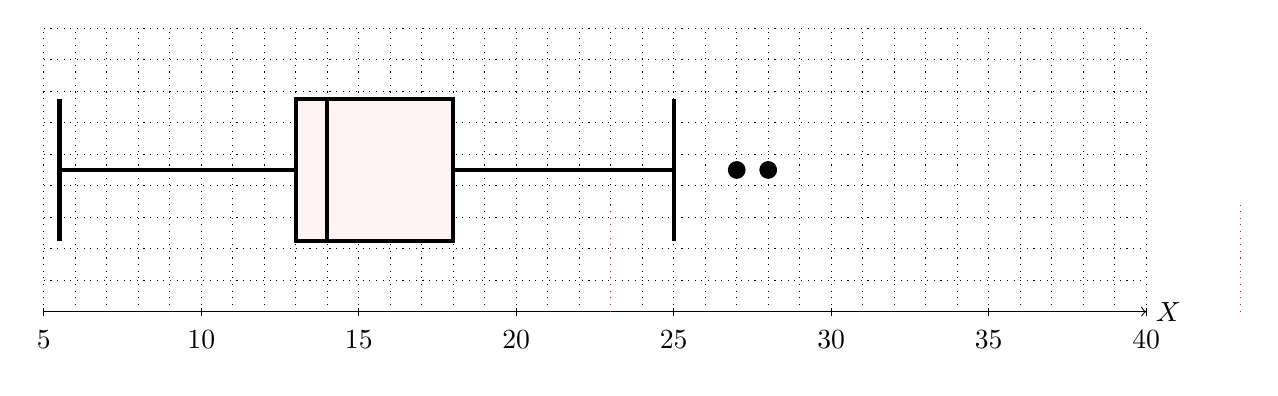
\begin{tikzpicture}[x=0.4cm,y=0.9cm]
         \draw[step=0.4cm,,dotted,color=black] (-5,0) grid (30,4);
		\draw[->] (-5,0) -- (30,0) node[right] {$X$} ;
		\draw[step=0.4cm,,dotted,color=red] (13,0) -- (13,1.5) node[above] { };
		\draw[step=0.4cm,,dotted,color=red] (33,0) -- (33,1.5) node[above] { };
		\foreach \X in {5,10,15,20,25,30,35,40} {
			\draw (\X-10,0.05cm) -- (\X-10,-0.05cm) node[below] {$\X\strut$};}
		\draw[ultra thick][fill=red!5] (3,1) rectangle (8,3);
		\draw[ultra thick] (-4.5,1) -- (-4.5,3);
		\draw[ultra thick] (-4.5,2) -- (3,2);
		\draw[ultra thick] (8,2) -- (15,2);
		\draw[ultra thick] (4,1) -- (4,3);
		\draw[ultra thick] (15,1) -- (15,3);
        \filldraw [black] (17, 2) circle (3pt);
        \filldraw [black] (18, 2) circle (3pt);
			\end{tikzpicture}\\
	\end{center}

\emptybox{9cm}

\begin{solution}
      \begin{eqnarray*}
		q_{0.25}= x_{(0.25\times 21+0.5)} &=& x_{(5,75)} \\
		&=& 13 \\
            q_{0.75}= x_{(0.75\times 21+0.5)} &=& x_{(16,25)} \\
		&=& 18 \\
            b_{inf} = q_{0.25} - 1.5 \times (q_{0.75}-q_{0.25})
            &=& 13 - 1.5 \times 5 \\
            &=& 5.5
\end{eqnarray*}   
La moustache de gauche sur le graphique devrait être placée à la plus petite valeur observée supérieure à la borne inférieure, donc à 11.
\end{solution}

\pagesuivante{\ref{micro}}
\newpage
\suite{\ref{micro}}

\part Vous apprenez que les trois plus grandes observations (25, 27, 28) sont erronées. Le nouveau jeu de données est donc:

\begin{center}
\begin{tabular}{  c c c c c c c c }
11  &11  &11  &12  &13  &13  &13 \\
13 &14  &14  &14  &14 &15 & 16 \\
16 & 18 & 18 & 19 &  & & \\
\end{tabular}
\end{center}

À partir de ce nouveau jeu de données, répondez aux questions suivantes. Nous nommons «jeu de données original» celui qui inclut les observations 25, 27 et 28.

\textbf{\textit{Inscrivez «Vrai» ou «Faux» dans les cases appropriées.}}

\begin{subparts}
\subpart[1]La médiane échantillonnale du nouveau jeu de données est inférieure ou égale à celle du jeu de données orginal.

\vfrep{}

\subpart[1] La moyenne échantillonnale du nouveau jeu de données est égale à celle du jeu de données original.

\vfrep{}

\subpart[1] La variance échantillonnale du nouveau jeu de données est inférieure à celle du jeu de données orignal.

\vfrep{}

\begin{solution}
    
    i. Vrai

    ii. Faux

    iii. Vrai
\end{solution}
   

\end{subparts}
\end{parts}


\newpage


%%%%%%%%%%%%%%%% QUESTION %%%%%%%%%%%%%%%%
\question\label{estimateursPonctuels} 

Soit $X_1, \dots, X_9$ un échantillon aléatoire d'une variable $X$ de loi Normale $\mathcam{N}(12, 4)$. Nous avons que $X_1, \dots, X_9$ sont indépendantes. 

\begin{parts}
    \part[5] Calculez la probablité que la moyenne échantillonnale soit supérieure à la vraie moyenne $\mu = 12$ par plus de 0,62 écarts-types échantillonnaux. Justifiez votre réponse.

    \emptybox{10cm}
    
    \begin{solution}
        \begin{align*}
            P(\overline{X} > \mu + 0,62S)
            &= P(\overline{X} - \mu  > 0,62S) \cr
             &= P\left(\frac{\overline{X} - \mu}{S/\sqrt{n}}  > \frac{0,62 S}{S/\sqrt{n}}\right) \cr
             &= P\left( T_{n-1} > 0,62 {\sqrt{9}}\right) \cr
             &= P\left( T_{8} > 1,86\right) \cr
             &= 0,05
        \end{align*}
    \end{solution}

    \part[4] Calculez la probabilité que la variance échantillonnale soit supérieure à 1,09. Justifiez votre réponse.

    \emptybox{10cm}
    
        \begin{solution}
        \begin{align*}
            P(S^2 > 1,09)
             &= P\left(\frac{(n-1)S^2}{\sigma^2}  > \frac{(n-1)1,09}{\sigma^2}\right) \cr
             &= P\left( \chi_{n-1}^2  > \frac{8\times 1,09}{4}\right) \cr
             &= P\left( \chi_{8}^2  > 2,18 \right) \cr
             &= 0,975
        \end{align*}
    \end{solution}
\end{parts}


\newpage

%%%%%%%%%%%%%%%% QUESTION %%%%%%%%%%%%%%%%
\question\label{cable} 
\bigskip
Le vérificateur interne d'une entreprise  a effectué une vérification du prix de 28 transactions choisies aléatoirement. Il a obtenu une  moyenne échantillonnale de 225\$ avec un écart-type échantillonnal de 20\$. On suppose que le prix d'une transaction est distribué selon une loi normale.

\begin{parts}
\part[6]  Calculez un intervalle de confiance pour la moyenne théorique du prix avec un niveau de confiance de 95\%. Justifiez votre réponse.
    
\emptybox{11cm}

\begin{solution}
On a $n=28,\;\overline{x}=225\$  \text{ et } s=20\$$, alors
    \begin{eqnarray*}
      IC_{\mu}(95\%)    &=& \left[\overline{x} - t_{0.025;27}\times \dfrac{s}{\sqrt{n}}\; ,\; \overline{x} + t_{0.025;27}\times \dfrac{s}{\sqrt{n}}\right] \\
                        && \\
                        &=& \left[225 - 2.052\times \dfrac{20}{\sqrt{28}} \; ,\; 225 + 2.052\times \dfrac{20}{\sqrt{28}}\right] \\
                        && \\
                        &=& \left[217.24 \; , \; 232.76\right].
    \end{eqnarray*}
\end{solution}


\part[3] Quelle est la marge d'erreur dans l'estimation de la moyenne théorique du prix, pour un niveau de confiance de 99\%. Justifiez votre réponse.

\emptybox{8cm}

\begin{solution}
On a aussi, $n=28,\; t_{0.005;27} = 2.771 \text{ et } s=20\$ $, alors, $\text{ Marge d'erreur } = 2.771 \times \dfrac{20}{\sqrt{28}} = 10.47$.
\end{solution}



\end{parts}

\end{questions}

\begin{center}

\includegraphics[page=1,scale=0.8]{Tables_lois.pdf}
\end{center}

\begin{center}

\includegraphics[page=2,scale=0.8]{Tables_lois.pdf}
\end{center}

\begin{center}

\includegraphics[page=3,scale=0.8]{Tables_lois.pdf}
\end{center}
\begin{center}


\includegraphics[page=4,scale=0.8]{Tables_lois.pdf}
\end{center}
\begin{center}


\includegraphics[page=5,scale=0.8]{Tables_lois.pdf}
\end{center}
\begin{center}


\includegraphics[page=6,scale=0.8]{Tables_lois.pdf}
\end{center}
\begin{center}


\includegraphics[page=7,scale=0.8]{Tables_lois.pdf}
\end{center}
\begin{center}


\includegraphics[page=8,scale=0.8]{Tables_lois.pdf}
\end{center}




\end{document} 


%\newpage
%\mbox{}
%\newpage


%%%%%%%%%%%%%%%% QUESTION SPPLÉMENTAIRE %%%%%%%%%%%%%%%%
%\question\label{cable} 


%La société ROULEMENTABILLE fabrique des roulements à billes. Les tolérances exigées pour un client, la DUPONT S.A., sont particulièrement draconiennes. Pour cette raison, un contrôle de qualité est effectué sur chaque bille avant livraison. La proportion de pièces ne satisfaisant pas aux spécifications de diamètre est de 10\% et la proportion de pièces présentant un défaut de forme est de 20\%.\\

%\begin{parts}
%\part[] Question a.

    %\bigskip

    %Le chef d'atelier estime que ces deux types de défaut sont indépendants. Si l'on suppose qu'il a raison, quelle est la proportion de pièces présentant au moins un défaut?

%\begin{solution}
%\begin{itemize}\itemsep10pt
       % \item[$\bullet$] Soient les événements $A$ = "défaut de diamètre" et $B$ = "défaut de forme".
      %  \item[$\bullet$] On sait que: $P(A) = 0.1,\; P(B) = 0.2$,\\ \ \\
      %   alors $P(A \cap B) = P(A) \times P(B)$ (car $A$ et $B$ sont supposés indépendants).
     %    Donc, \begin{eqnarray*}
      %            P(A \cup B)  &=& P(A) + P(B) - P(A \cap B) \\
     %             &=& P(A) + P(B) – P(A) \times P(B) \\
      %            &=& 0.1 + 0.2 – (0.1 \times 0.2) \\
      %            &=&  0.28.
     %          \end{eqnarray*}
  %  \end{itemize}
 %   La proportion de pièces présentant au moins un défaut est de \textbf{28\%}.
%\end{solution}


%\vspace{1cm}
%\part[] Question b.

\bigskip
%Le directeur de la fabrication n'est pas d'accord. Lorsque les pièces présentent un défaut de forme, alors dans 30\% des cas les pièces présentent un diamètre non conforme aux spécifications. Si l'on suppose que le directeur a raison, quelle est la nouvelle proportion de pièces présentant au moins un défaut?    

%\begin{solution}
%\begin{itemize}\itemsep10pt
 %           \item[$\bullet$] On nous indique que $P(A | B) = 0.3$. Alors,
 %                           \begin{eqnarray*}
  %                            P(A \cap B)  &=& P(A | B) \times P(B) \\
   %                                     &=& 0.3 \times 0.2 \\
    %                                    &=& 0.06
     %                       \end{eqnarray*}
      %       À la lumière de cette nouvelle information, On recalcule $P(A \cup B)$:
       %                     \begin{eqnarray*}
        %                      P(A \cup B)  &=& P(A) + P(B) - P(A \cap B) \\
         %                               &=& 0.1 + 0.2 – 0.06 \\
          %                              &=& 0.24
           %                 \end{eqnarray*}
        %\end{itemize}
       % La proportion de pièces présentant au moins un défaut est de \textbf{24\%}.
%\end{solution}


%\end{parts}


%\newpage
%\mbox{}
%\newpage

%\end{questions}



%%%%%%%%%%%%%%%% QUESTION %%%%%%%%%%%%%%%%
\question[3]\label{probabilite} 

On considère une expérience aléatoire dont deux événements  $A$ et $B$ sont tels que:\\ $P(A) = 0.3 \text{ et } P(A \cup B) = 0.7$.\\ 

Calculer $P(\overline{B}|\overline{A})$. Justifiez votre réponse.\\

\emptybox{15cm}

\begin{solution}
\begin{eqnarray*}
   P(\overline{B}|\overline{A})      &=&  \dfrac{P(\overline{B}\cap \overline{A})}{P(\overline{A})}\\
                                    &=&  \dfrac{P(\overline{B\cup A})}{1-P(A)}\\
                                    &=&  \dfrac{1-P(B\cup A)}{1-P(A)}\\
                                    &=&  \dfrac{1-0.7}{1-0.3}\\
                                    &=&  \dfrac{3}{7} .
\end{eqnarray*}
\end{solution}




\newpage